\documentclass{article}
\usepackage{graphicx}
\usepackage[margin=1.5cm]{geometry}
\usepackage{amsmath}

\begin{document}
\twocolumn

\title{Monday warm-up: Forces II and Forces III}
\author{Prof. Jordan C. Hanson}

\maketitle

\section{Memory Bank}

\begin{itemize}
\item Newton's Second Law: $\vec{F}_{net} = m\vec{a}$. (The net external force on an object is equal to the mass of the object times the acceleration of the object).
\item The horizontal force of friction: $\vec{f} = - \mu N \hat{i}$.  $N$ is the magnitude of the normal force.
\end{itemize}

\section{Forces, II}

\begin{enumerate}
\item In Fig. \ref{fig:1}, a man with mass $m$ and weight $w$ stands on a scale in an elevator.  Which of the followinng is true, if the elevator is accelerating upwards?
\begin{itemize}
\item A: $w = mg$
\item B: $w < mg$
\item C: $w > mg$
\item D: $w = 0$
\end{itemize}
\item Suppose the man's mass is $60$ kg.  He is standing on a scale in an elevator that is \textit{accelerating upwards} at $0.2$ m/s$^{2}$.  What is the weight on the scale? \\ \vspace{2cm}
\item Assume there is a force of friction on $m_1$ in Fig. \ref{fig:3}.  Derive an expression for the acceleration of $m_2$. \\ \vspace{2cm}
\item Let $m_1 = 200$ grams, $m_2 = 50$ grams, and the coefficient of friction be $\mu = 0.1$.  What is the acceleration of $m_2$?  Assume the string tension is constant.
\end{enumerate}

\begin{figure}
\centering
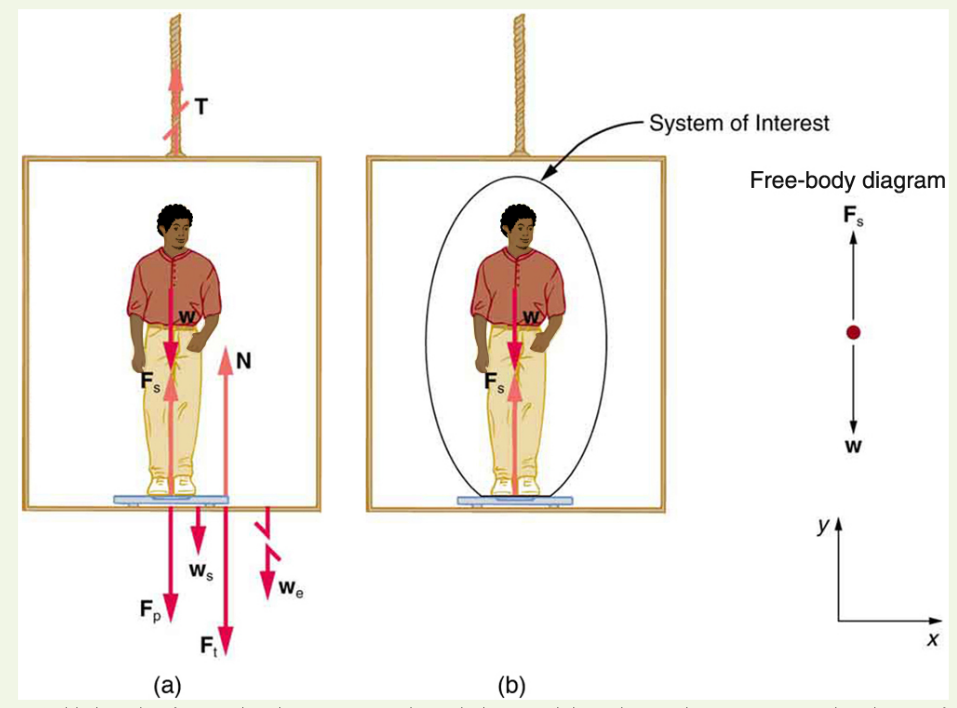
\includegraphics[width=0.35\textwidth,trim=13cm 0cm 0cm 0cm,clip=true]{figures/elevator.png}
\caption{\label{fig:1} A person on a scale in an elevator.}
\end{figure}

\begin{figure}
\centering
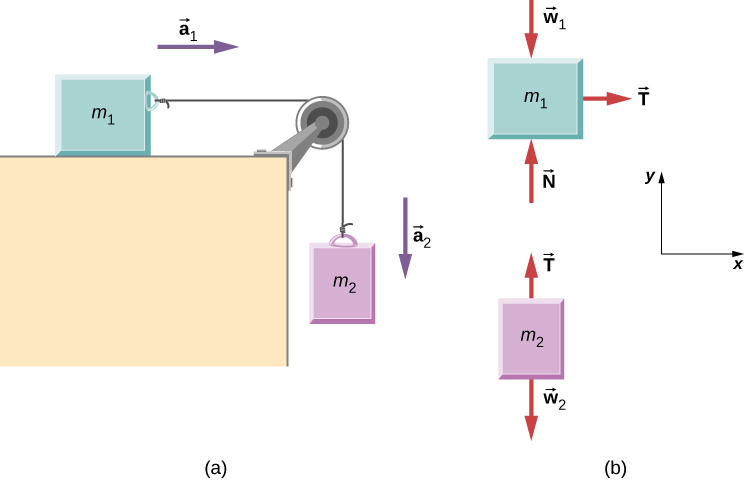
\includegraphics[width=0.45\textwidth]{figures/blocks.jpg}
\caption{\label{fig:3} Friction acts on block $m_1$ and gravity acts on $m_2$.  Note that the force of friction does not appear in the free-body diagram.  We must add friction, $\vec{f}$, to $m_1$.}
\end{figure}

\end{document}
